\documentclass[10pt]{beamer}
\setbeamertemplate{note page}[plain]
\usepackage[utf8]{inputenc}
\usepackage[T1]{fontenc}
\usepackage[utopia]{mathdesign}
\usetheme[progressbar=frametitle]{metropolis}




\usepackage{amsmath}
\usepackage[spanish, mexico]{babel}
\usepackage{graphicx}
% \usepackage{xcolor}
\usefonttheme[onlymath]{serif}
\usepackage{natbib}

% Footnotes.
% \makeatother
% \renewcommand{\thefootnote}{\ifcase\value{footnote}\or$\dagger$\or
% $\ast$\or\$\or\#\or\ddagger\or$\therefore$\fi}
% \makeatletter


\title{Gimballed EDF propelled VTVL \\ 
vehicle design and control}
\subtitle{Defensa de proyecto final}
\date{\today} 
\author{Patricio Whittingslow \\ Luís Cretton}

% !TeX root = ../main.tex



%% ROCKET
\newcommand{\CG}{{\mathrm{CG}}}
\newcommand{\LCG}{L_\CG}
\def\equilibrium{\mathrm{eq}}


%% DIFFERENTIAL OPERATOR
\makeatletter
\providecommand*{\diff}%
{\@ifnextchar^{\DIfF}{\DIfF^{}}}
\def\DIfF^#1{%
	\mathop{\mathrm{\mathstrut d}}%
	\nolimits^{#1}\gobblespace}
\def\gobblespace{%
	\futurelet\diffarg\opspace}
\def\opspace{%
	\let\DiffSpace\!%
	\ifx\diffarg(%
	\let\DiffSpace\relax
	\else
	\ifx\diffarg[%
	\let\DiffSpace\relax
	\else
	\ifx\diffarg\{%
	\let\DiffSpace\relax
	\fi\fi\fi\DiffSpace}

%% CONTROL:
\newcommand{\dimfont}[1]{\ensuremath{#1}}
\newcommand{\Cme}[1]{\mathbf{#1}}
\newcommand{\Mme}[1]{\mathbf{#1}}
\newcommand{\Nme}[1]{\mathrm{#1}}
\newcommand{\Ts}{T_s}

\newcommand{\eye}{\Mme{I}}
%transpose
\def\dt{\Delta t}
\def\tp{\!^{\top}\!}
% Small
\def\MA{\Mme{A}}
\def\MB{\Mme{B}}
\def\MC{\Mme{C}}
\def\MD{\Mme{D}}
\def\ME{\Mme{E}}

\def\MQ{\Mme{Q}}
\def\MR{\Mme{R}}
\def\MK{\Mme{K}}
\def\MW{\Mme{W}}
\def\MX{\Mme{X}}
\def\MV{\Mme{V}}
\def\ctrb{\Mme{Y}}
\def\Mzero{\Mme{0}}
\def\obsv{\Mme{\mathcal{O}}}

\newcommand{\ts}[2]{\left. #1\right|_{ #2}}

\def\error{\varepsilon}
\def\Cx{\Cme{x}}
\def\Cf{\Cme{f}}
\def\Cy{\Cme{y}}
\def\Cu{\Cme{u}}
\def\Cn{\Cme{n}}
\def\Cd{\Cme{d}}
\def\Czero{\Cme{0}}
\def\Cv{\Cme{v}}
\def\Cz{\Cme{z}}
\def\Cw{\Cme{w}}

\def\Jcost{\Cme{\mathcal{J}}}
% RK4
\def\Ca{\Cme{a}}
\def\Cb{\Cme{b}}
\def\Cc{\Cme{c}}


\def\noise{{n}}
\def\disturb{{d}}
\newcommand{\di}{\ensuremath{\textrm{d}}}

\newcommand{\Matlab}{{\sc Matlab}}

\def\matdiv{\bm{\textbackslash}}

\newcommand{\spartial}[2]{\frac{\partial {#1}}{\partial {#2}}}
\newcommand{\dpartial}[2]{\frac{\partial^2 #1}{\partial #2 ^2}}

%# ROBUST
\def\lap{\mathcal{L}}
\newcommand\lapc[1]{\lap \left\{#1\right\}}
\newcommand\ilapc[1]{\lap^{-1} \left\{#1\right\}}
\def\xbar{\bar{x}}
\def\ubar{\bar{u}} 

\def\MP{\Mme{P}}
\def\ML{\Mme{L}}
\def\MT{\Mme{T}}
\def\MS{\Mme{S}}


\def\Cr{\Cme{r}}
\def\Cn{\Cme{n}}

\def\openloop{{\textrm{\tiny{LA}}}}
\def\closedloop{{ \textrm{\tiny{LC}}}}
\def\true{{ \textrm{\tiny{real}}}}

% RIGID BODY MECHANICS
\newcommand{\frm}[1]{\mathrm{#1}}  % Frame of reference
\newcommand{\ogn}[1]{\mathcal{#1}} % Frame origin / point of reference
\newcommand{\skw}[1]{\tilde{#1}}   % skew matrix notation
\newcommand{\uveci}{{\bm{\hat{\textnormal{\bfseries\i}}}}}
\newcommand{\uvecj}{{\bm{\hat{\textnormal{\bfseries\j}}}}}
\DeclareRobustCommand{\uvec}[1]{{% Unit length vector of arbitrary orientation
		\ifcsname uvec#1\endcsname
		\csname uvec#1\endcsname
		\else
		\bm{\hat{\mathbf{#1}}}%
		\fi
}}
\DeclareRobustCommand{\avec}[1]{{%
		\underline{#1} %		\bm{\mathbf{#1}}%
}}
\DeclareRobustCommand{\bvec}[1]{{% Orthogonal basis vector
%		\ifcsname bvec#1\endcsname
%		\csname bvec#1\endcsname
%		\else
		\bm{\hat{\mathbf{#1}}}%
%		\fi
}}
\def\tform{\mathbf{A}}
\newcommand{\transform}[1]{\tform^\frm{#1}}
\newcommand{\dottransform}[1]{\dot{\tform}^\frm{#1}}
\def\attitude{\mathbf{H}}
\newcommand{\inertia}[2]{J_{\ogn{#1}}^{\frm{#2}}}
\newcommand{\inertiarotor}[2]{\inertia{\!\mathrm{r}#1}{#2}}


\makeatletter
\newcommand*\bigcdot{\mathpalette\bigcdot@{.5}}
\newcommand*\bigcdot@[2]{\mathbin{\vcenter{\hbox{\scalebox{#2}{$\m@th#1\bullet$}}}}}
\makeatother

% THEOREMS/ EXERCISES
\usepackage{amsthm}
\theoremstyle{definition}
%\newtheorem{definition}{Definition}[chapter]
%\newtheorem{theorem}{Teorema}[chapter]
%\newtheorem{exercise}{Ejercicio}[chapter]

\begin{document}

\maketitle

\begin{frame}{Objetivo}
    \begin{itemize}
        \item Tecnología central para el desarrollo aeroespacial futuro
        \item Desarrollo de vehículo plataforma para ensayos a pequeña escala
    \end{itemize}

    \hspace{0.7cm}
    \begin{figure}[htb]
        \centering
        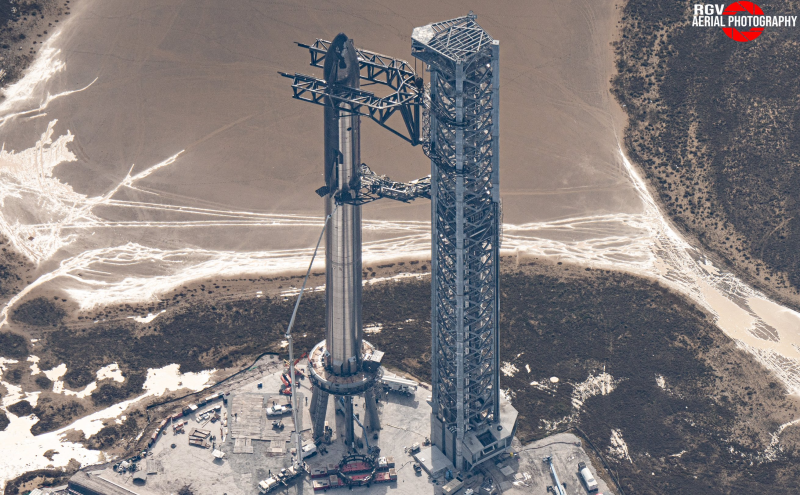
\includegraphics[width=0.6\linewidth]{fig/starship.png}
        \caption{Starship: referente en tecnología de vehículos orbitales reutilizables.}
        \label{fig:starship}
    \end{figure}
\end{frame}

\begin{frame}{Estado del arte}
    \begin{itemize}
        \item Tecnología monorrotor fijo tiene uso amplio
    \end{itemize}

    \begin{figure}[htb]
        \centering
        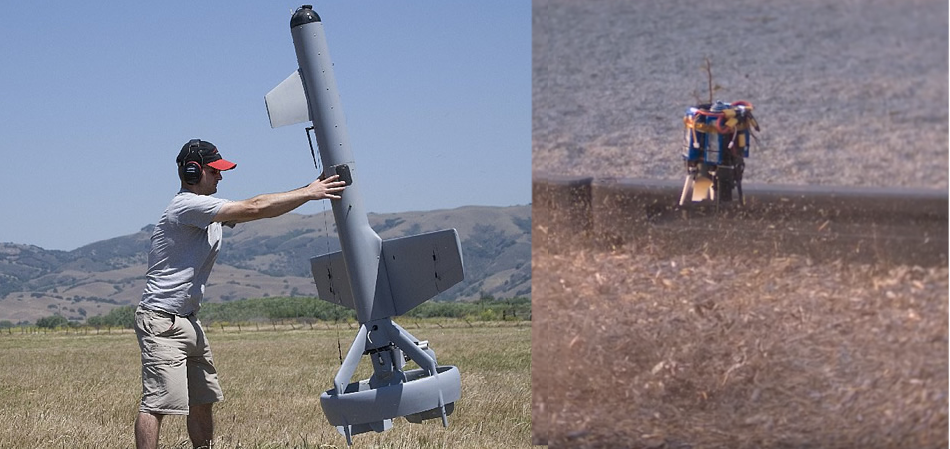
\includegraphics[width=0.8\linewidth]{fig/vbat_icarus.png}
        \caption{Dos vehículos VTVL eléctricos modernos. ``VBat'' (Izq.) y ``\href{https://hackaday.com/2018/08/31/single-rotor-drone-a-thrust-vectoring-monocopter/}{Ikarus}''.}
        \label{fig:vbat_icarus}
    \end{figure}
\end{frame}

\begin{frame}{Estado del arte}
    \begin{itemize}
        \item Tecnología monorrotor para empuje vectorial siendo usado por la ESA para ensayar algoritmos de control.
    \end{itemize}

    \begin{figure}[htb]
        \centering
        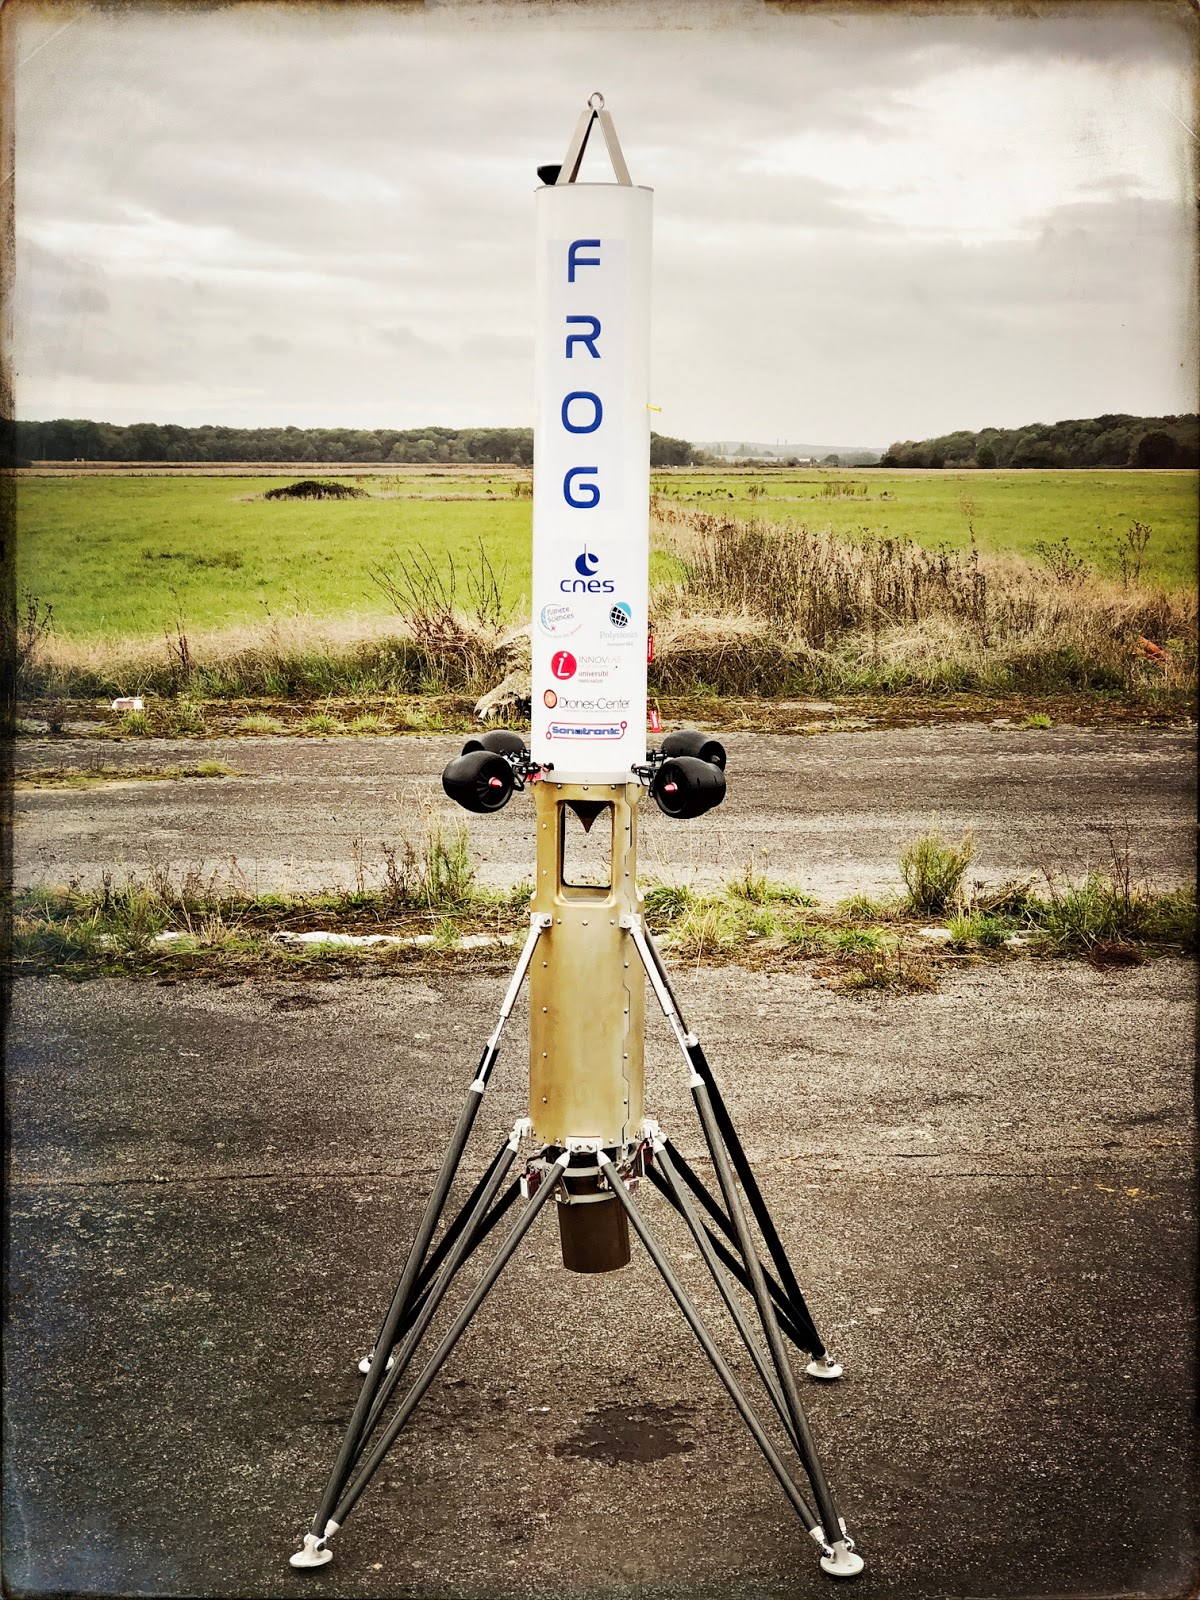
\includegraphics[height=5cm]{fig/frog_esa.jpg}
        \caption{FROG de la ESA. Plataforma de ensayo de sistemas.}
        \label{fig:frog_esa}
    \end{figure}
\end{frame}

\section{Diseño}

\begin{frame}{Diseño -- Propulsión másica}
    \begin{itemize}
        \item Agua
        \item Peróxido HTP y cama catalítica
    \end{itemize}
    \begin{figure}[!ht]
        \centering
        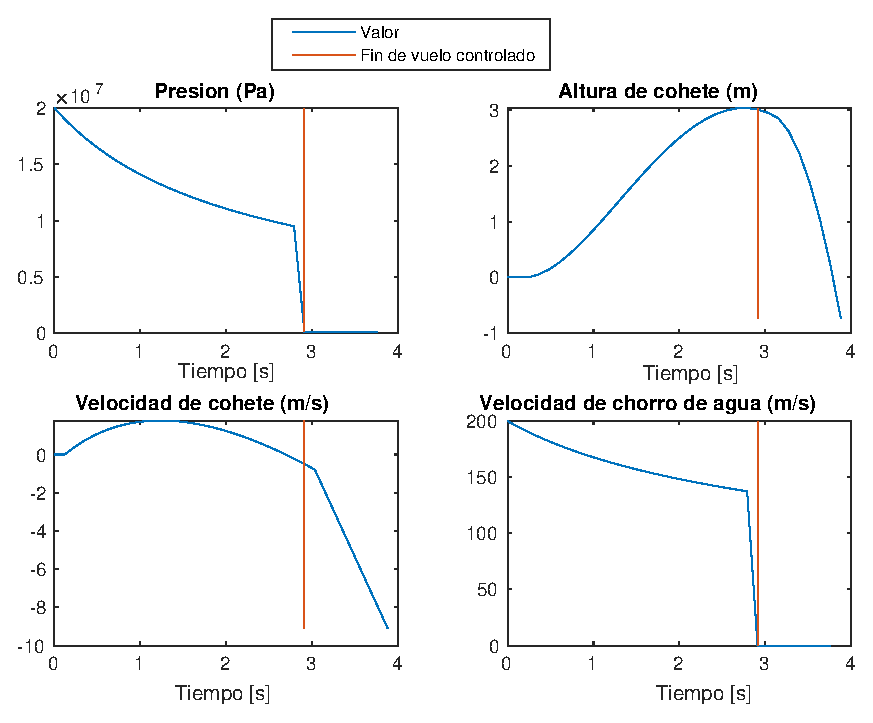
\includegraphics[width=0.6\linewidth]{fig/bottlerocket}
        \caption{Análisis preliminar para un vehículo propulsado por agua a presión. La presión es la del tanque (absoluta). El peso estructural que se utilizó fue de 10kg.}
        \label{fig:bottlerocket}
    \end{figure}
\end{frame}

\begin{frame}{Diseño -- Elección de propulsor}
    \begin{table}[!ht]
        \centering
        \begin{tabular}{l|r|r|r}
    Diámetro de EDF    & \multicolumn{1}{l|}{70mm} & \multicolumn{1}{l|}{90mm} & \multicolumn{1}{l}{120mm} \\ \hline
        Masa estructural {[}kg{]}           & 0,4                       & 1                         & 2                          \\ \hline
        Masa batería       {[}kg{]}                 & 0,9                       & 1,9                       & 2                          \\ \hline
        Mas electrónica {[}kg{]}            & 0,5                       & 1                         & 1                          \\ \hline
        Empuje restante {[}kgf{]}           & 0,01                      & 0,478                     & 3,116                      \\ \hline
        Tiempo vuelo {[}s{]}                & 253              & 184              & 132                \\ \hline
        Precio baterías-propulsor {[}usd{]} & 165                   & 365                   & 693                   \\ \hline
        Costo total {[}ars{]}               & 23968              & 53017              & 101313                 \\ \hline
        \end{tabular}
        \caption{Estudio de diferentes EDF's disponibles en el mercado. El requerimiento excluyente para la selección de batería fue que permita vuelo sostenido por 2 minutos.}
        \label{tab:edfseleccion}
    \end{table}
\end{frame}

\section{Simulación}

\begin{frame}{Simulación -- Modelo matemático}
    Notación y tratamiento matemático de \cite{hahn2013rigid}.
    
    \begin{figure}[htb!]
        \centering
        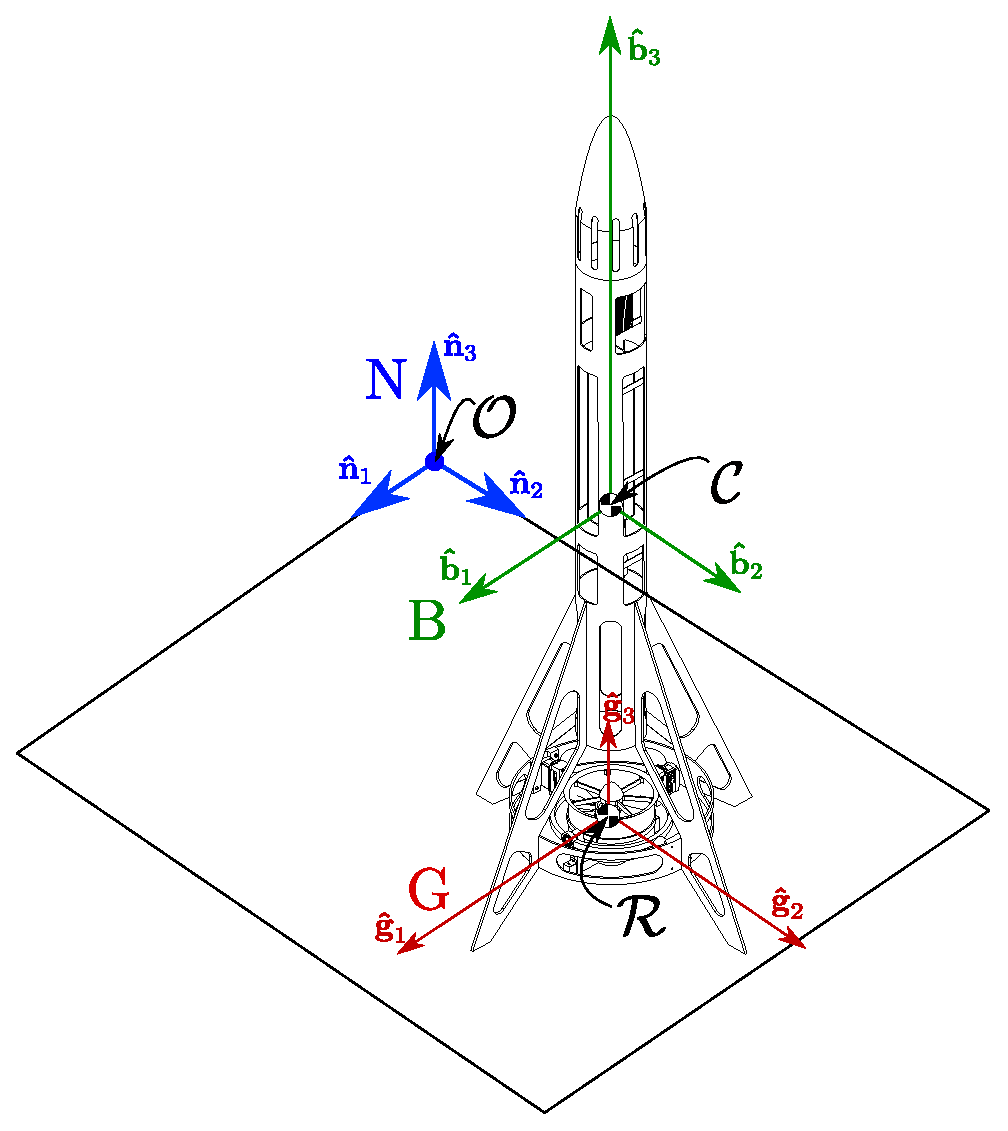
\includegraphics[width=0.5\textwidth]{fig/marcosDiagrama.eps}
        %\caption{Marcos de referencia tomados para el análisis de cuerpo rígido. Por simplicidad se toman los centros de masa del cardán y del rotor como coincidentes en el punto $\ogn{R}$.}
    \end{figure}
\end{frame}

\begin{frame}{Simulación -- Modelo matemático}
    Aceleración angular del vehículo tomando en cuenta efecto giroscopo y fuerzas externas debido a vorticidad.
    \begin{align*}
        {}^\frm{B}\frac{\di }{\di t} \left(\avec{\omega}_\frm{BN}^\frm{B} \right) = & \left(\inertia{C}{B}\right)^{-1} \cdot  \left( - \skw{\avec{\omega}}_\frm{BN}^\frm{B} \cdot \inertia{C}{B}\cdot \avec{\omega}_{\frm{BN}}^{\frm{B}} - \transform{{BG}} \cdot\skw{\avec{\omega}}_\frm{GB}^\frm{G} \cdot \inertiarotor{R}{G}  \cdot \avec{\omega}_r^\frm{G} - \right.\\
     & \left.\skw{\avec{\omega}}_\frm{BN}^\frm{B} \cdot \inertiarotor{R}{G}  \cdot \avec{\omega}_r^\frm{G} -  \transform{{BG}}\cdot  \inertiarotor{C}{G} \cdot  {}^\frm{N} \dot{\avec{\omega}}_{\!r}^{\frm{G}} + \avec{M}_\ogn{C}^\frm{B} \right)
     \end{align*}
\end{frame}

\begin{frame}{Simulación -- Control}
    \begin{itemize}
        \item Representación espacio de estados.
        \item Controlador LQR.
        \item Estimador de actitud Madgewick.
    \end{itemize}
    \begin{align}
        \dot{\Cx} &= \Mme{A} \Cx + \Mme{B} \Cu \\
        \Cu &= \Mme{K}_{\textrm{LQR}} \left(\Cx-\Cx_0 \right)
    \end{align}
\end{frame}

\bibliography{tex/biblio} % Indica archivo
\bibliographystyle{plainnat} %estilo de bibliografía

\end{document}